\chapter[Probability Distribution Map and Task-Difficulty Map Editor Interface]{Probability Distribution Map and Task-Difficulty Map Editor Interface}
\label{chap:MapEdit}

%=====================================================================================================
\section{Introduction}
\label{introduction7}


At the \textbf{between-episodes} scale, a searcher might have additional case-specific information (e.g, past experience, knowledge of the search area or weather conditions, or the profile of the missing person) and would like to modify the general plan produced at the strategic scale. Moreover, as search progresses, the search plan should change due to newly found evidence (or the lack of it) from either the ground searchers or previous UAV flights. We developed two autonomy management tools at this scale that allow the user to manage two types of information: the \textit{probability distribution map} and the \textit{task-difficulty map}.

\begin{figure}
\centering
\begin{tabular}{cc}
	\begin{minipage}{0.45\textwidth}
	\centering
	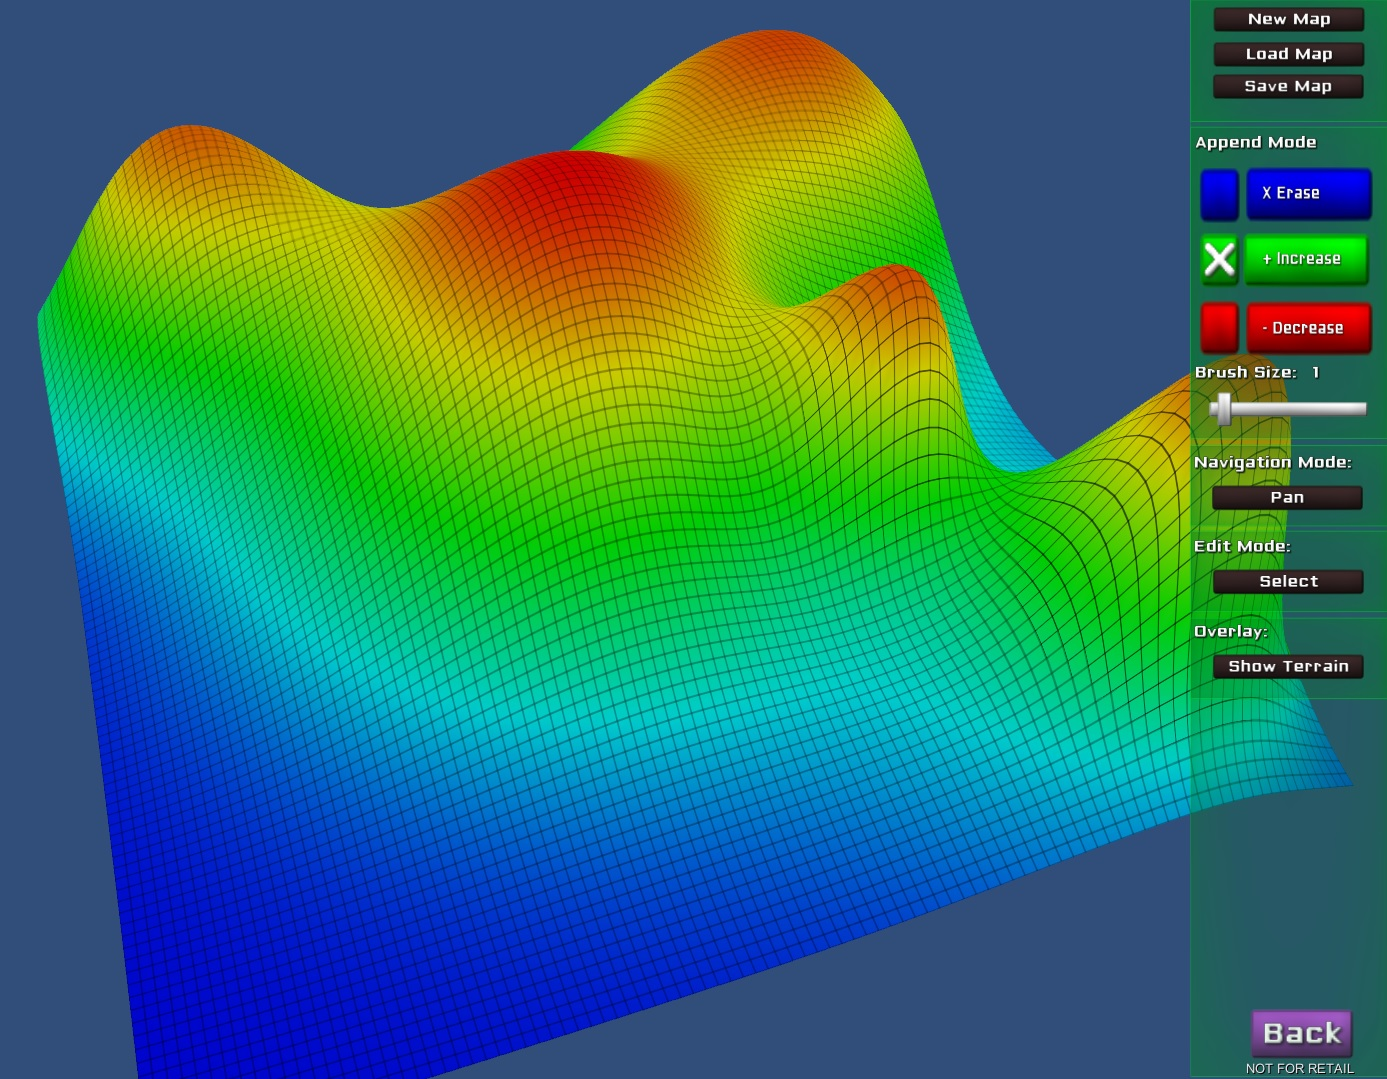
\includegraphics[width=2.8in]{DistEditExample.jpg}
	\caption{An example \textit{probability distribution map} generated using the \textbf{DistEdit} tool.}
	\label{DistEditExample2}
	\end{minipage}
&
	\begin{minipage}{0.45\textwidth}
	\centering
	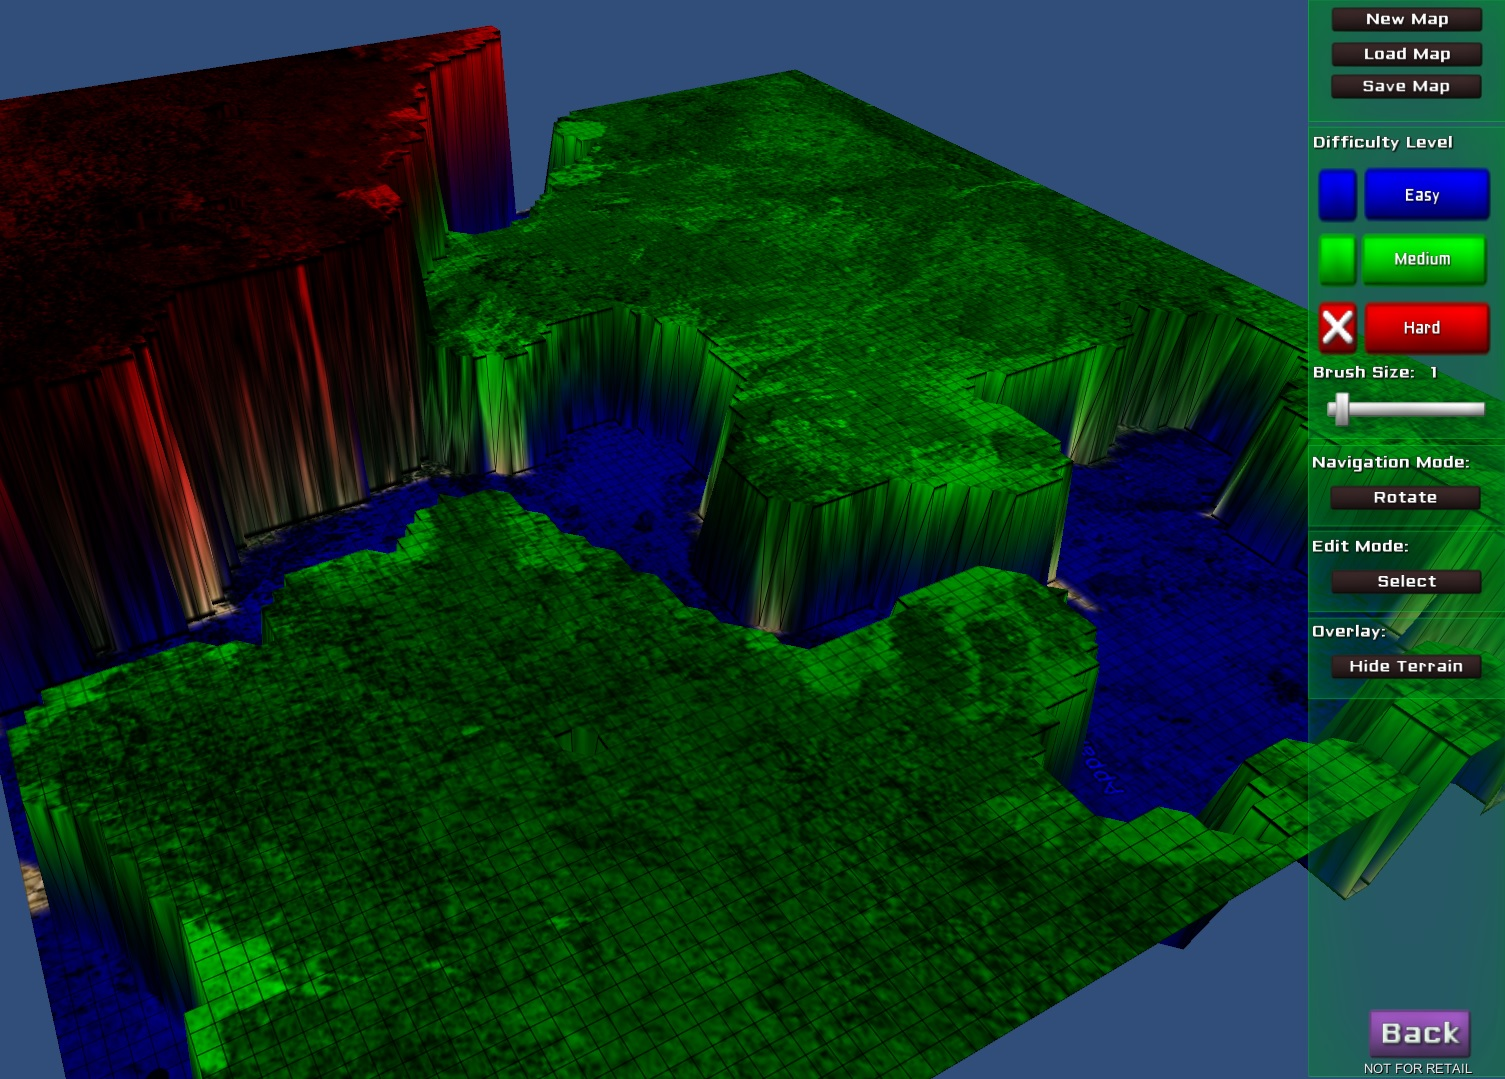
\includegraphics[width=2.8in]{DiffEditExample.jpg}
	\caption{An example \textit{task-difficulty map} generated using the \textbf{DiffEdit} tool with a satellite image of the search region overlaid on top.}
	\label{DiffEditExample2}
	\end{minipage}
\end{tabular}
\end{figure}

Searchers can use the \textbf{DistEdit} tool to modify a \textit{probability distribution map} and use the \textbf{DiffEdit} tool to modify a \textit{task-difficulty map} generated at the \textbf{strategic} scale. Both tools enable the user to view maps as 3D surfaces where a color map is applied for better distinction (red means high probability area or high task-difficulty level and blue means low). The user can use mouse and finger gestures to rotate/pan/zoom the respective map and edit the shapes of the maps in 3D to incorporate information that the autonomous components are unable to interpret. The user also has the option to overlay a satellite image of the search area on top of the maps for better alignment and precision.

If the user is dissatisfied with the \textit{probability distribution map} or \textit{task-difficulty map} systematically generated at the \textbf{strategic} scale, using the \textbf{DistEdit} and \textbf{DiffEdit} tools he or she can also create a \textit{probability distribution map} and/or a \textit{task-difficulty map} from scratch. Figure~\ref{DistEditExample2} and~\ref{DiffEditExample2} show screen captures of these two tools and also example maps generated using the two tools.

Both tools enable the searchers to incorporate additional information only available to or understandable by the user into the two information representations -- in the form the autonomous components of the UAV system can understand -- and then interactively use the UAV path-planner to use the additional information produce highly efficient paths. We designed both tools to support common touch-screen finger gestures. The user has the option to perform all tasks using only finger gestures, only keyboard/mouse controls, or a hybrid of the two.

%=====================================================================================================
\section{The DiffEdit Tool}
\label{DiffEdit}

The \textbf{DiffEdit} tool enables the user to create or modify a \textit{task-difficulty map} by marking areas with different levels of difficulty. When using a UAV to support WiSAR, task difficulty is related to sensor detection probability. A difficult area on the map represents a place where the likelihood of detecting the missing person is low (maybe due to terrain features, vegetation density, or lighting conditions). By marking an area with high task difficulty, the user can indirectly tell the UAV to make multiple passes in the area, or avoid the area and set high priority to areas marked with low task difficulty. When combined with a prior probability, encoded as a \textit{probability distribution map}, an area with medium probability and low task difficulty may be more attractive than an area with high probability but high task difficulty.

%===================================================
\subsection{Editing vs. Starting New}

The tool is modular for easy integration into the overall intelligent system. A \textit{task-difficulty map} is stored as an external file, and can be loaded (imported) into the tool. A modified map can be saved (exported) to the hard drive. The group of buttons on the upper right corner of Figure~\ref{DiffEdit003} are for this purpose.

\begin{figure}
\centering
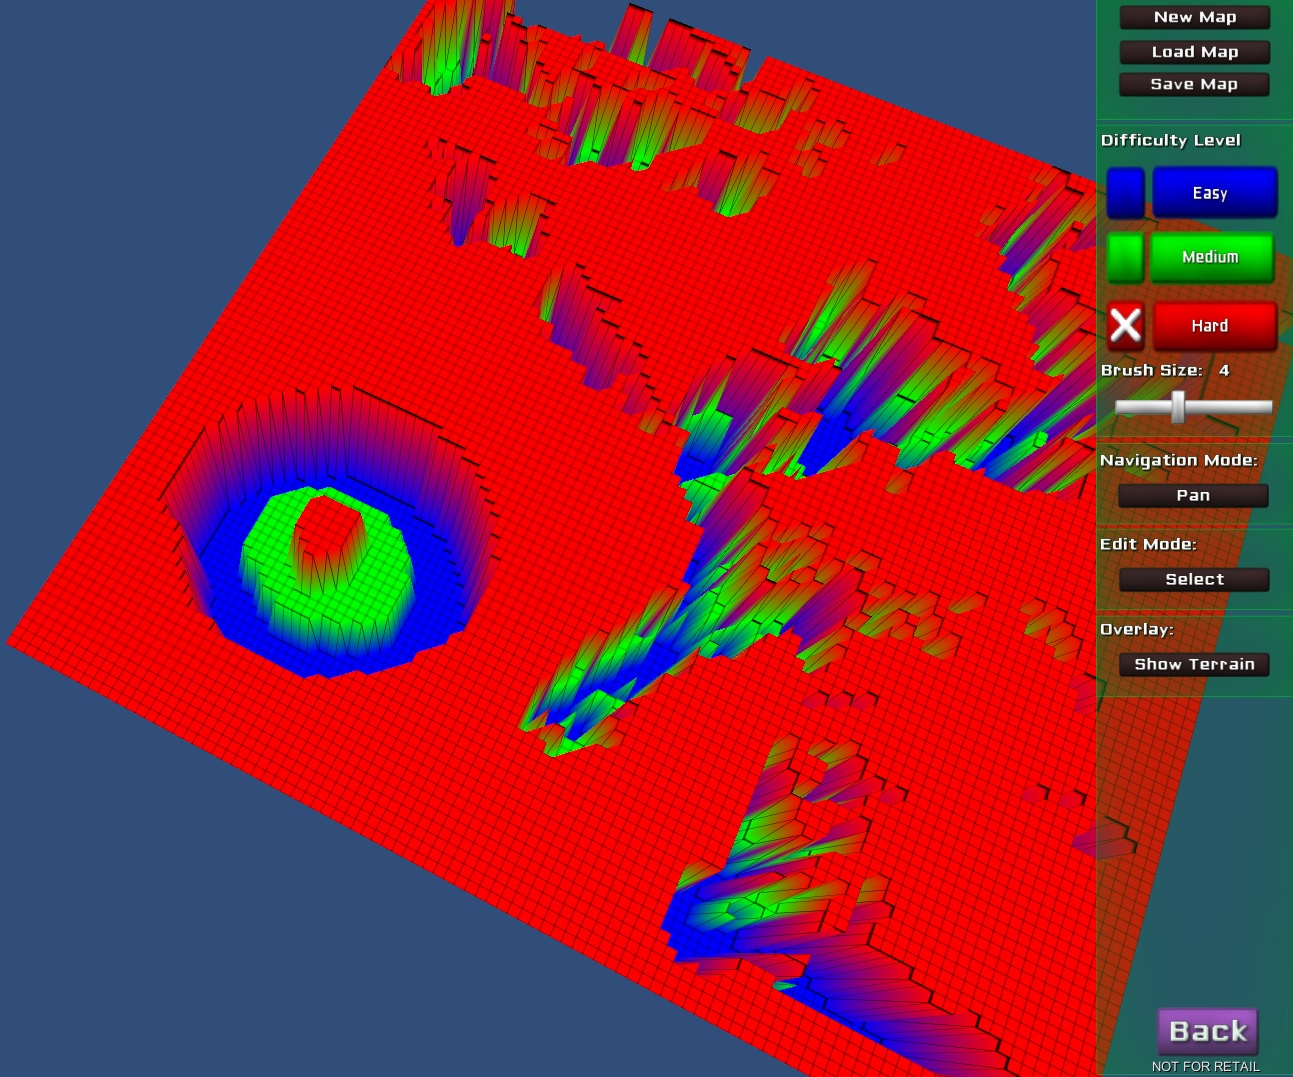
\includegraphics[width=5.25in]{DiffEdit003.JPG}
\caption{An example \textit{task-difficulty map} systematically generated at the \textbf{strategic} scale for a real WiSAR scenario with modification made on the lower left corner using the \textbf{DiffEdit} tool.}
\label{DiffEdit003}
\end{figure}

The user can click the \textbf{New Map} button to start a map from scratch, if the user is dissatisfied with the systematically generated map from the \textbf{strategic} scale. The \textbf{Load Map} button lets the user load an existing map. This map could be from the \textbf{strategic} scale, or could be from a UAV flight episode in the \textbf{between-episodes} scale, so information collected from the previous UAV flight could be incorporated into the map. 

In Figure~\ref{DiffEdit003}, the right part of the map is systematically generated from vegetation density information at the \textbf{strategic} scale where the red plateau areas are areas with high vegetation density. The canyon shapes indicate areas with sparse vegetation density. The circular hole on the lower left corner of the map shows user-made modifications to the systematically generated map using the \textbf{DiffEdit} tool. Then the user can click the \textbf{Save Map} button to store the map as an file externally.

The tool also lets the user overlay satellite imagery of the search area on top of the \textit{task-difficulty map} for better reference and precision (Figure~\ref{DiffEdit001} shows an example). What image to use can be configured in tool settings. Then the user can click the overlay button \textbf{Show Terrain} (\textbf{Hide Terrain}) to toggle back and forth.

%===================================================
\subsection{3D Navigation Controls}

The \textbf{DiffEdit} tool is a true 3D environment where the \textit{task-difficulty map} is shown as a 3D surface. Task difficulty is represented by both height and color (blue is easy, green is medium, and red is hard). The ability to rotate the surface in 3D and zoom in/out allows the user to get a good grip of task difficulty in different areas of the search region.

The user can click the navigation mode toggle button to switch between \textbf{Rotate} mode and \textbf{Pan} mode. In the \textbf{Rotate} mode, the user can use the arrow keys and the WASD keys to rotate the map both vertically and horizontally in 3D. In the \textbf{Pan} mode, the arrow keys and the WASD keys can pan the map left-right and up-down. Finally, the mouse scroll wheel can be used to zoom the map in or out.

With a touch-screen device, buttons can be pressed with simple finger touches. A common two-finger rotate gesture will rotate the map; moving two fingers toward the same direction will pan the map to that direction; and the two-finger pinch gesture lets the user zoom the map in or out.

Using the rotate/pan/zoom function, the user has total control of the 3D environment. With the satellite imagery of the search area overlaid on top, the user can easily mark task difficulty at the desired resolution and precision.

\begin{figure}
\centering
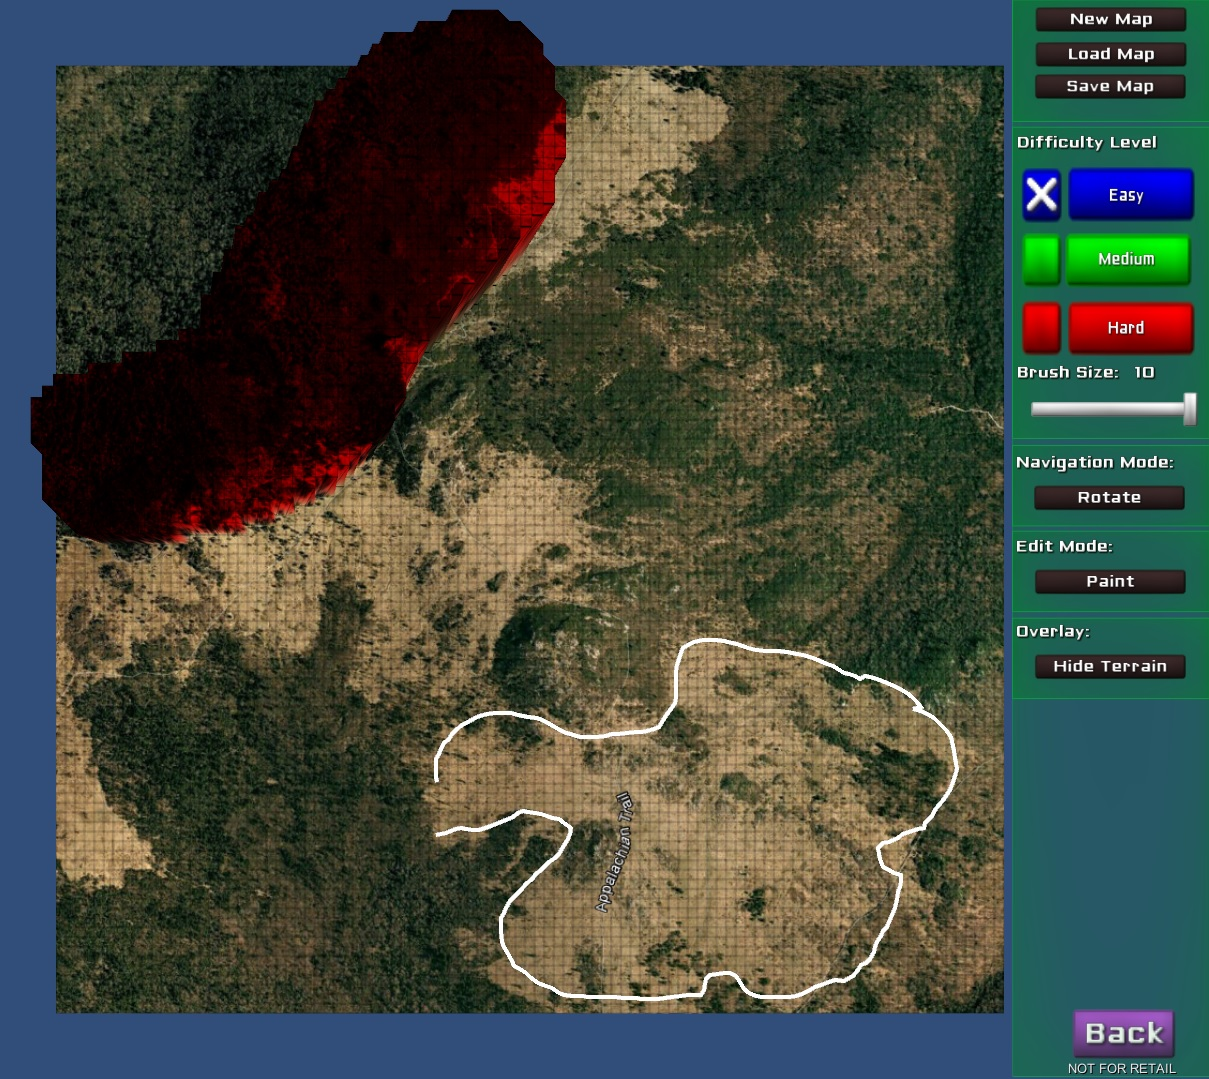
\includegraphics[width=6in]{DiffEdit001.JPG}
\caption{A satellite imagery of the search area loaded into the \textbf{DiffEdit} tool as an overlay, an example high task-difficulty area on the top left corner made using the paintbrush tool, and an example selection made using the lasso selection tool.}
\label{DiffEdit001}
\end{figure}


%===================================================
\subsection{Paint Mode vs. Lasso Select Mode}

The \textbf{DiffEdit} tool lets the user edit a \textit{task-difficulty map} using two modes: the \textit{paint} mode and the lasso \textit{select} mode. The user can select which mode to use by clicking the toggle button \textbf{Paint} (\textbf{Select}). First the user needs to select a desired task difficulty level by clicking one of the difficulty level buttons. The tool supports three task difficulty levels: easy, medium, and hard. Each task difficulty level is represented on the 3D \textit{task-difficulty map} by color and height. The easy level (color blue and low height) could represent an area with no vegetation coverage or sparse type vegetation (e.g., grass). The medium level (color green and medium height) could mean the area is covered by plants such as short shrubs. The hard level (color red and high height) might be used to mark areas with dense forest (e.g., evergreen type plants). Although the tool only supports three task difficulty levels presently, it can be easily extended to support more difficulty levels through, for example, a slider bar.

In the \textbf{paint} mode, the cursor becomes the brush and is shown as a circular shadow projected onto the 3D surface from above, with its color matching the selected task-difficulty level. The user can move the brush size slider in the control panel (see the right side of Figure~\ref{DiffEdit001}) to select a desired brush size between 1 and 10. The size of the brush is indicated on the map by the radius of the circular shadow. Then the user can mark task difficulty on the \textit{task-difficulty map} by painting different areas using the paintbrush. If a satellite imagery is overlaid on top of the \textit{task-difficulty map}, the zoom function described in the previous section can be combined with different brush size selection to achieve the level of precision desired by the user. Figure~\ref{DiffEdit001} shows an example where an area on the satellite imagery with dense vegetation (upper left part of the map) is marked with high task difficulty (red) using the paintbrush tool.

In the \textbf{select} mode, the user can drag a freehand selection around the desired area. The tool will automatically connect the starting point and the end point of the line to form a closed selection, and the selected area is automatically marked with the selected task difficulty level. The white line in Figure~\ref{DiffEdit001} shows an area selected by a user, and Figure~\ref{DiffEdit002} shows how the selected area is automatically marked with the selected easy task difficulty.

Similarly, using a touch-screen device, the user can use a finger to paint on top the \textit{task-difficulty map} in the \textbf{paint} mode. The user can also use a finger to draw freehand selection on the map to select an area in the \textbf{select} mode.


\begin{figure}
\centering
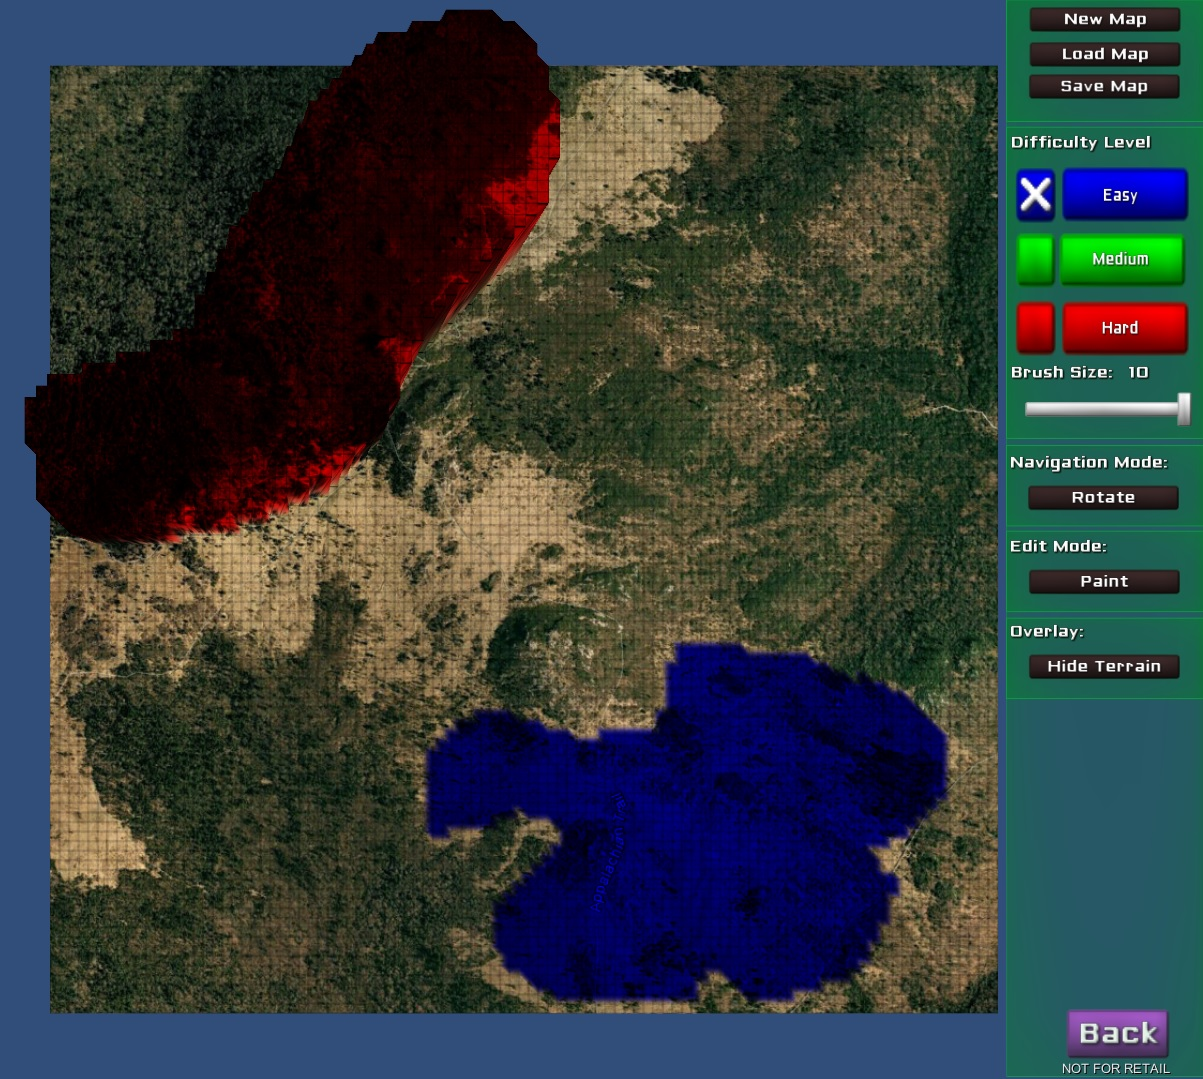
\includegraphics[width=6in]{DiffEdit002.JPG}
\caption{The area selected in Figure~\ref{DiffEdit001} is automatically marked with the selected task difficulty level easy.}
\label{DiffEdit002}
\end{figure}

%=====================================================================================================
\section{The DistEdit Tool}
\label{DistEdit}

The \textbf{DistEdit} tool enables the user to create or modify a \textit{probability distribution map} by adding or subtracting Gaussian distributions. This way the user can generate a mixture of Gaussians to represent the desired probability distribution, which is common in real WiSAR operations.  When using a UAV to support Wilderness Search and Rescue (WiSAR), a \textit{probability distribution map} shows the place where the missing person is likely to be found. The modified probability distribution can be used later by the path planner to prioritize tasks and plan UAV paths. By marking an area as a high priority area, the searchers can indirectly manipulate the UAV to search the area before other areas without the need to manually specify waypoints.

\begin{figure}
\centering
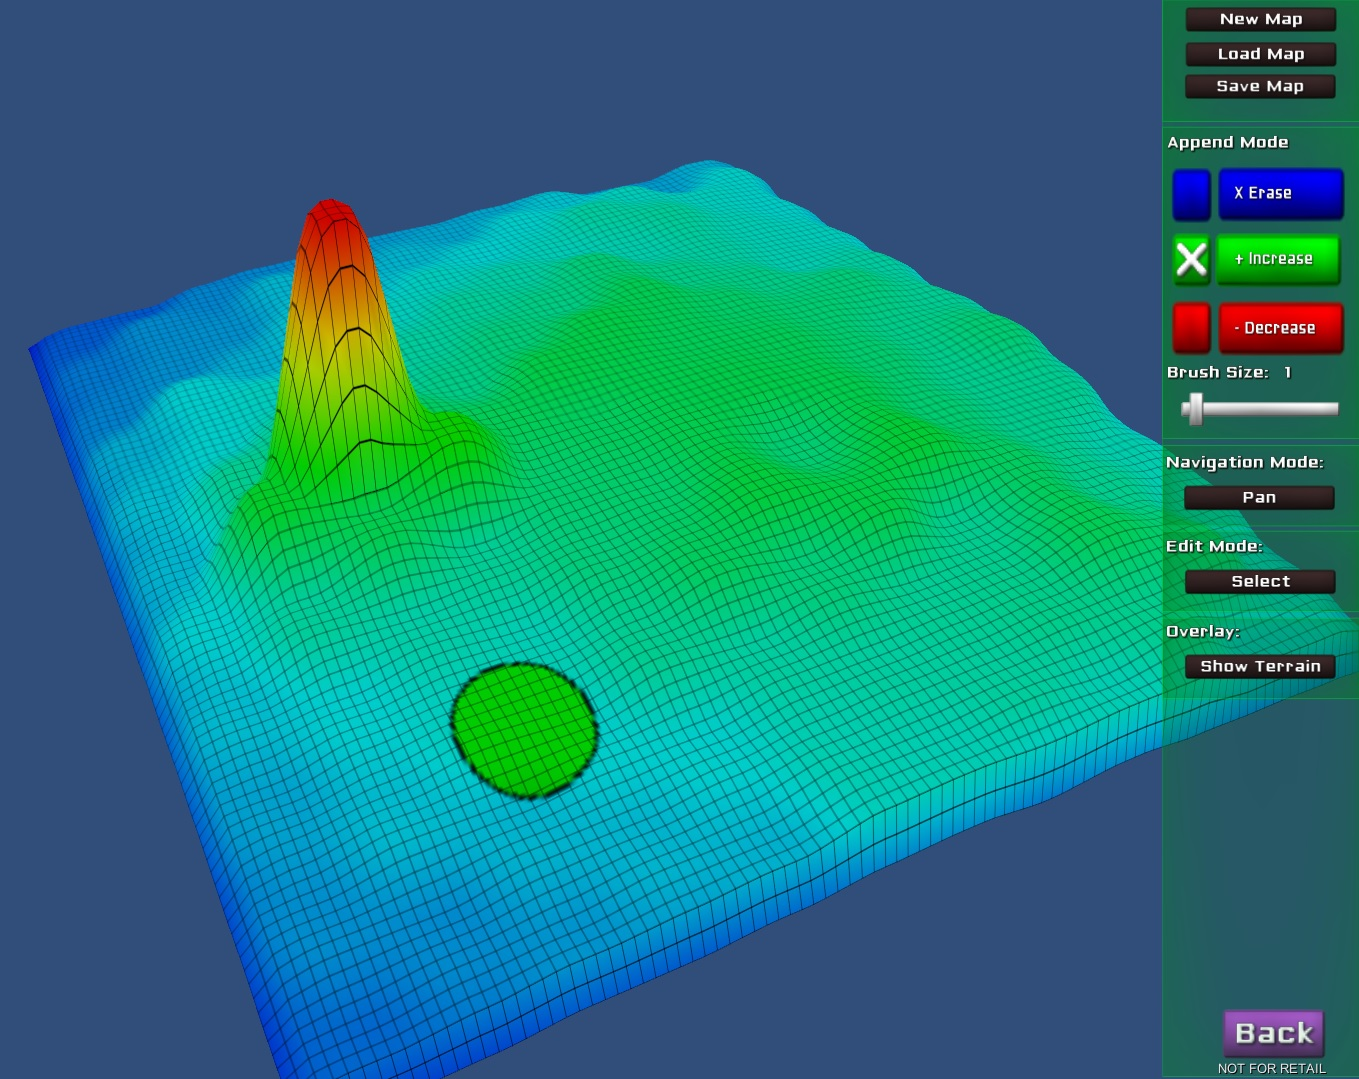
\includegraphics[width=6in]{DistEdit004.JPG}
\caption{An example \textit{probability distribution map} systematically generated using the \textbf{DistCreate} tool at the \textbf{strategic} scale for a real WiSAR scenario.}
\label{DistEdit004}
\end{figure}

%===================================================
\subsection{Editing vs. Starting New}

Similar to the description of the \textbf{DiffEdit} tool used to modify the \textit{task-difficulty map}, the \textbf{DistEdit} tool is modular and the \textit{probability distribution map} is stored as an external file. The user can load a \textit{probability distribution map} systematically generated at the \textbf{strategic} scale using the \textbf{DistCreate} tool and improve it, or start from scratch if the user is dissatisfied with the automatically generated map. This map can then be updated after each UAV flight episode as more information is collected in the previous flight. Areas already covered by the UAV can be marked with lower probability; areas where possible evidence has been found by the UAV or ground searchers can be marked with high probability. 

The group of buttons are identical to the \textbf{DiffEdit} tool (\textbf{New Map}, \textbf{Load Map}, and \textbf{Save Map}) and the user also can similarly overlay satellite imagery on top of the \textit{probability distribution map}. Figure~\ref{DistEdit004} shows an example probability distribution systematically generated by the \textbf{DistCreate} component at the \textbf{strategic} scale. This map was generated using the HikerPaul WiSAR scenario~\cite{Lin2014Hierarchical} from the International Search \& Rescue Incident Database (ISRID)~\cite{Koester2008Lost}. The probability hill on the left side of the map indicates an area where the probability of finding the missing person is very high. The \textit{probability distribution map} is encoded with a color map where red indicates high probability areas and blue indicates low probability areas. Figure~\ref{DistEdit003} shows a \textit{probability distribution map} with satellite imagery overlaid on top of the map.

%===================================================
\subsection{3D Navigation Controls}

The 3D navigation controls in the \textit{DistEdit} tool is identical to the \textit{DiffEdit} tool described in the previous section. Arrow keys and the WASD keys are used to rotate the map vertically and horizontally in the \textbf{Rotate} mode and pan the map left-right and up-down in the \textbf{Pan} mode, and finger gestures on a touch screen device perform identical functions as the \textbf{DistEdit} tool. Mouse scroll wheel can be used to zoom the map in or out.

\begin{figure}
\centering
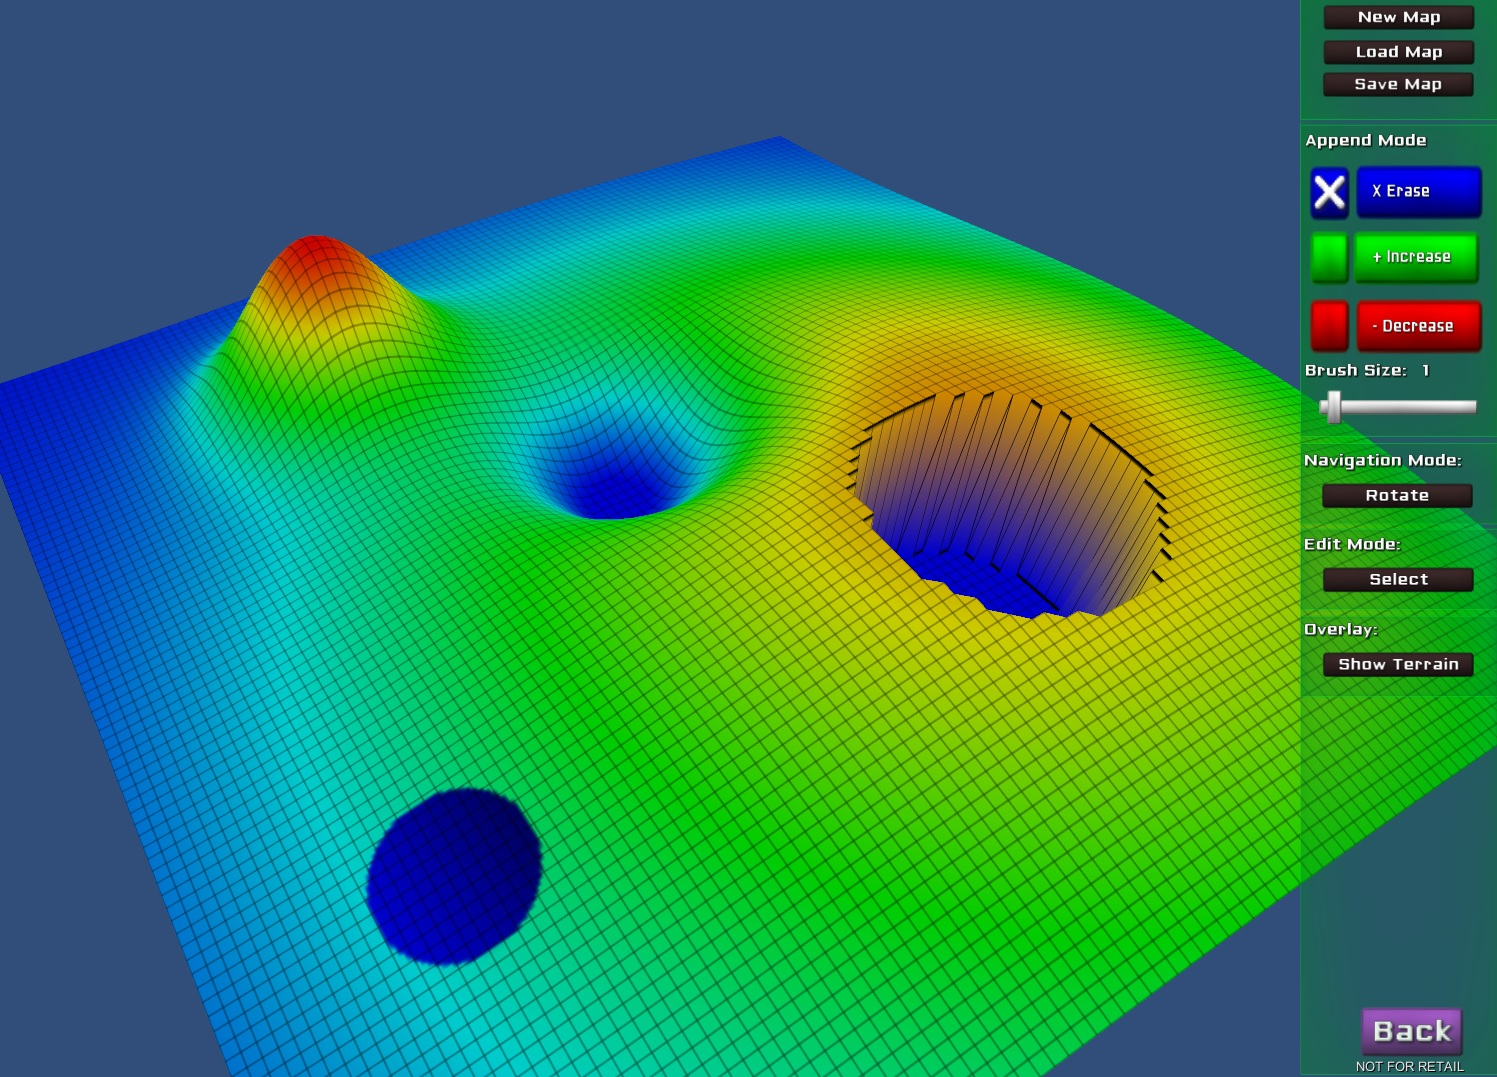
\includegraphics[width=5in]{DistEdit001.JPG}
\caption{An example \textit{probability distribution map} demonstrating how a Gaussian can be added to or subtracted from the map and how probability in an area can be completely erased.}
\label{DistEdit001}
\end{figure}

%===================================================
\subsection{Paint Mode vs. Lasso Select Mode}

The \textbf{DistEdit} tool lets the user edit a \textit{probability distribution map} using two modes: the \textit{paint} mode and the lasso \textit{select} mode. The user can select which mode to use by clicking the toggle button \textbf{Paint} (\textbf{Select}). 

In the \textbf{paint} mode, the user can choose to add a Gaussian to (or subtract a Gaussian from) the current \textit{probability distribution map} or erase the probability in an area. The user first clicks one of the three color coded buttons, \textbf{Erase}, \textbf{Increase}, and \textbf{Decrease}, then paints on the map using the paintbrush to make modifications.

If \textbf{Erase} is selected, painting an area on the map means completely erasing the probability in that area. This can be useful when an area has already been throughly searched by the UAV and/or ground searchers in the previous episode and the user is confident that the missing person is not in that area. The user can also move the cursor to paint with freehand. The brush size can be set using the brush size slider on the control panel. The big circular hole in Figure~\ref{DistEdit001} shows an example of an erased area created by using a paintbrush of the same size.

\begin{figure}
\centering
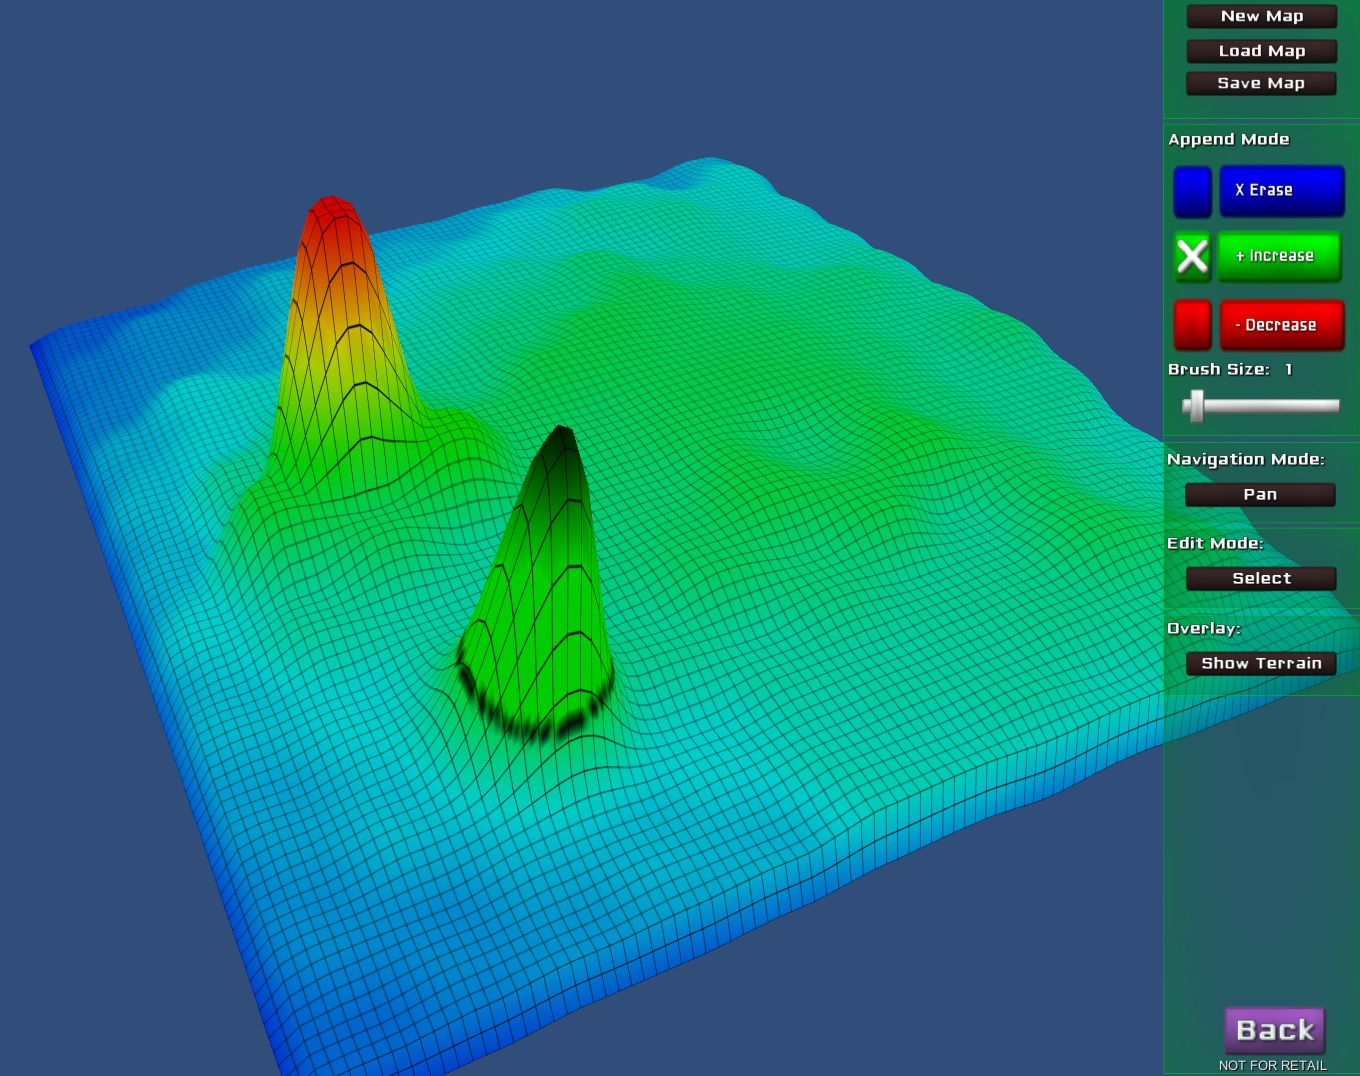
\includegraphics[width=6in]{DistEdit005.JPG}
\caption{A Gaussian is added to the systematically generated \textit{probability distribution map} shown in Figure~\ref{DistEdit004}.}
\label{DistEdit005}
\end{figure}

If \textbf{Increase} is selected, The brush size determines the standard deviation (with a radius equivalent to three times the standard deviation) of a symmetric Gaussian to be added to the existing \textit{probability distribution map}. The mouse click (or finger press gesture) position determines the mean of the Gaussian distribution, and the duration of the click (or finger press gesture) determines the scale (height relative to other parts of the distribution) of the Gaussian distribution. The probability hill in Figure~\ref{DistEdit001} shows an example of a Gaussian added to the \textit{probability distribution map}. Figure~\ref{DistEdit005} shows how another probability hill can be added to the systematically generated \textit{probability distribution map} from the \textbf{strategic} scale. The black circle shows the brush size.

\begin{figure}
\centering
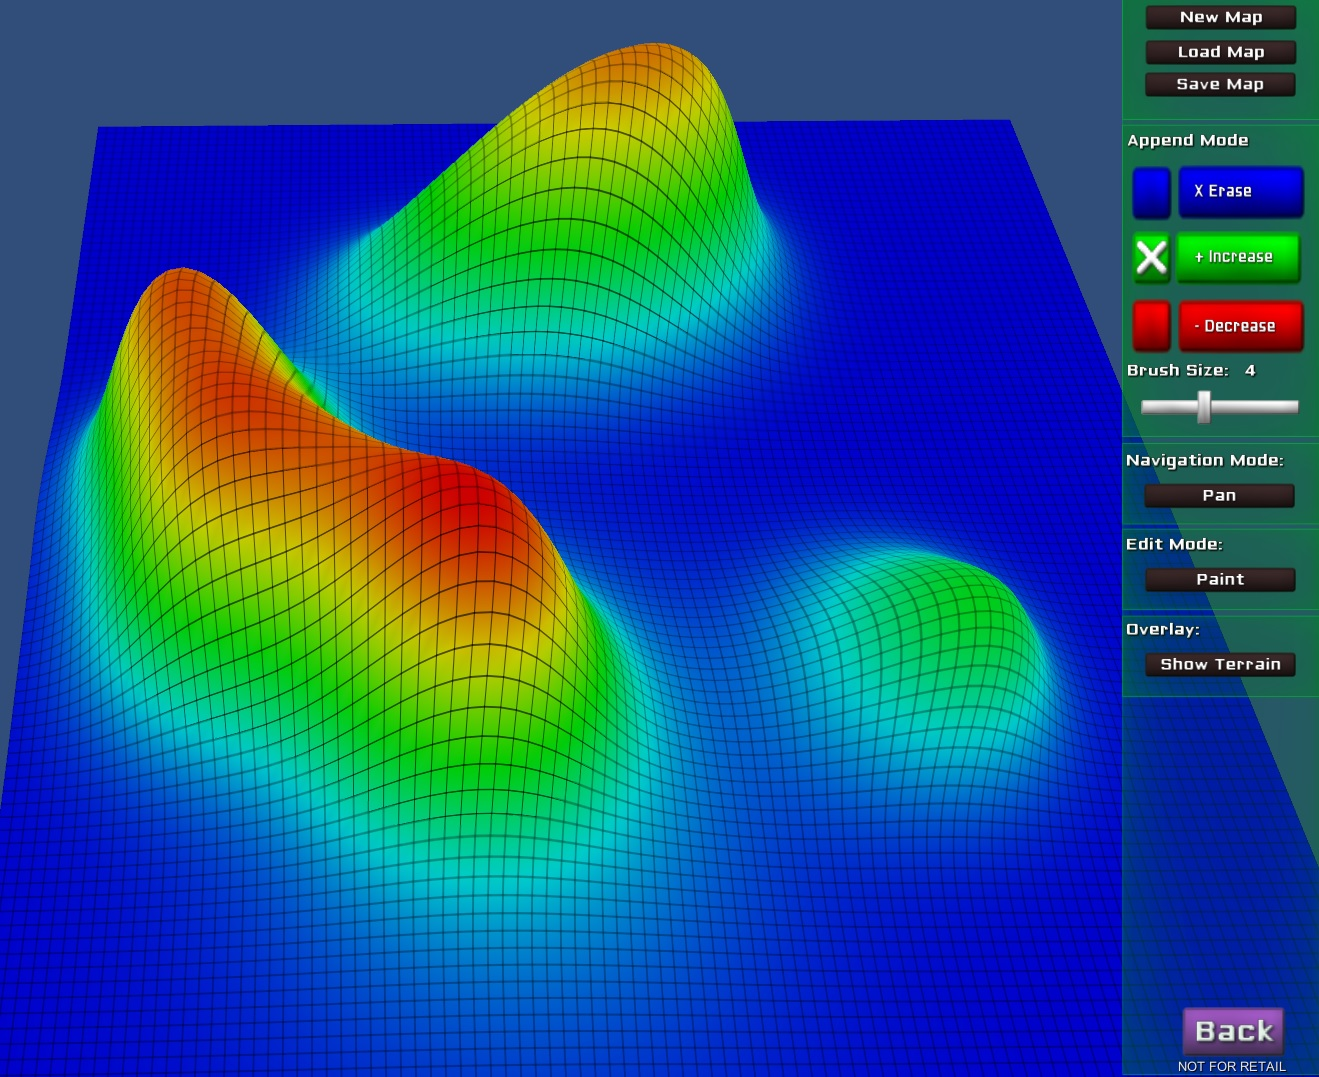
\includegraphics[width=6in]{DistEdit002.JPG}
\caption{Examples of ellipsically-symmetric and bivariate Gaussians and asymmetric bivariate distributions approximated using the \textbf{DistEdit} tool.}
\label{DistEdit002}
\end{figure}

If \textbf{Decrease} is selected, the effect is just the reverse of \textbf{Increase}. Instead of adding a Gaussian to the existing distribution map, a Gaussian is subtracted. The mean, standard deviation, and the scale of the Gaussian is determined the same way as mentioned above. The small basin in the middle of Figure~\ref{DistEdit001} shows an example of a Gaussian subtracted from the \textit{probability distribution map}.

The blue circle on the lower left part of the map in Figure~\ref{DistEdit001} shows the paintbrush cursor projected onto the 3D surface from above, so the user can see directly the brush size with respect to the entire map. The color of the circle matches the color-coded buttons in the control panel, so it is easy to tell which action (erase, increase, and decrease) is currently selected. The user can move the brush size slider in the control panel (see the right side of Figure~\ref{DiffEdit001}) to select a desired brush size between 1 and 10. The probability hill in Figure~\ref{DistEdit003} is created with brush size 10.

It is worth mentioning that although in the \textbf{paint} mode, only circularly-symmetric bivariate Gaussians (standard bivariate Normals) can be added to or subtracted from the \textit{probability distribution map}, ellipsically-symmetric bivariate Gaussians and asymmetric bivariate distributions can also be approximated using the paintbrush tool. For example, the user can create three circularly-symmetrical Gaussians where the means of these Gaussians are on a straight line with equal distance, the two Guassians on the outside have identical scales, and the Gaussian in the middle have a larger scale. The mixture of these three Gaussians approximates the shape of an ellipsically-symmetrical bivariate Gaussian. The user can also move the cursor in a straight line but in varying speed while adding a Gaussian to the map to approximate asymmetric bivariate distributions. Figure~\ref{DistEdit002} shows examples of such approximations.

Similar to the function in the \textbf{DiffEdit} tool, in the \textbf{select} mode the user can drag a freehand selection around the desired area. The tool will automatically connect the starting point and the end point of the line to form a closed selection. Probability in the selected area is automatically erased. The white line in Figure~\ref{DistEdit003} shows an area selected by a user. When satellite imagery of the search area is overlaid on top of the \textit{probability distribution map}, the user can zoom in using 3D controls and then trace an area on the satellite imagery using this method.

With both the \textbf{paint} mode and the \textbf{select} mode, when a touch-screen device is used, the user can use a finger to paint or select on top the \textit{task-difficulty map}.

%===================================================
\subsection{Cross-Platform Support}

Both the \textbf{DiffEdit} tool and the \textbf{DistEdit} tool are developed using the free version of the Unity Game Engine. This means that these tools are cross platform and can support Windows, Mac, Unix, and can be ported to mobile devices such as iPhone, iPad, Android tablets, and Android phones. Both tools also have web versions that can run under typical web browsers such as Chrome, Firefox, IE, and Safari. The platform independence adds value to these tools and make it more feasible to integrate the tools into real WiSAR operations.

\begin{figure}
\centering
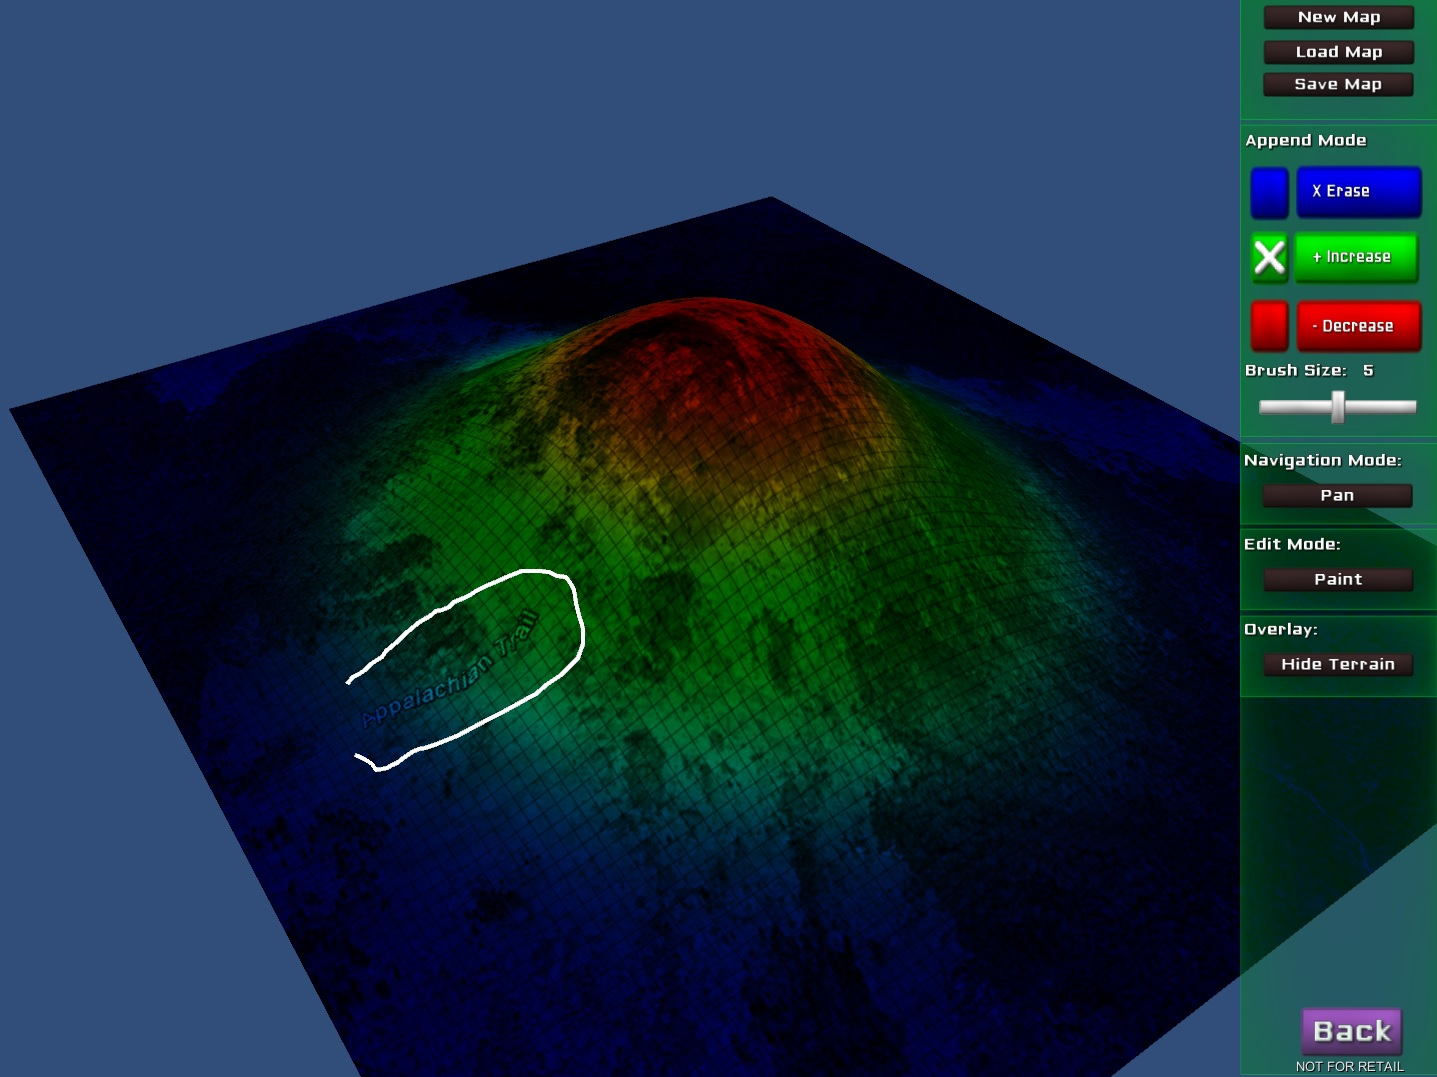
\includegraphics[width=6in]{DistEdit003.JPG}
\caption{An example \textit{probability distribution map} with the satellite imagery overlaid on top where an area is selected in the lasso \textbf{select} mode.}
\label{DistEdit003}
\end{figure}
